\documentclass[german,a5paper, twoside]{scrreprt} %report veraltet, scrreprt neu
%Packages
\usepackage{geometry} %Definition Satzspiegel
\geometry{left=2cm,right=2cm,top=2.1cm,bottom=2.2cm} 
\usepackage[ngerman]{babel}%auch für Umlaute???
\usepackage{bibgerm}%deutsche trennung
\usepackage[utf8]{inputenc}%Zeichensatz
\usepackage[T1]{fontenc}%fontsatz
\usepackage{geometry}
\geometry{a5paper}
\usepackage{setspace} 
\usepackage{musixtex} 
\usepackage{musixguit}
\usepackage{graphicx} %Graphiken
\usepackage{float}
\usepackage{placeins}
\usepackage{pdfpages}%mehrseitige PDFs einbinden
\usepackage{fancyhdr}%Kopfzeilen usw.
\usepackage{tikz}

\newcommand{\chort}[2]{\chord{\textbf{#1}}{#2}}
%\newcommand{\Liedname}{Fruehlingserwachen}
%\newcommand{\Abstand}{5mm}

\newcommand{\Liedname}{Du-hast-die-Wahl}
\newcommand{\Abstand}{8cm} %statt der 5cm einfach einen Abstand eingeben, damit der Text nicht mehr über den Noten ist. Faustregel: ungefähr 1.25cm pro Notenzeile

\newcommand{\Lizenz}{CC-BY-SA} %ist Standardmäßig eine CC4.0-BY-SA Lizenz. Wenn das nicht gewollt ist, CC-BY-SA einfach entfernen.



\usepackage{hyperref}

\begin{document}
\pagestyle{empty}
\begin{tikzpicture}[remember picture,overlay]
\node[anchor=north west,inner sep=5pt] at (current page.north west)
{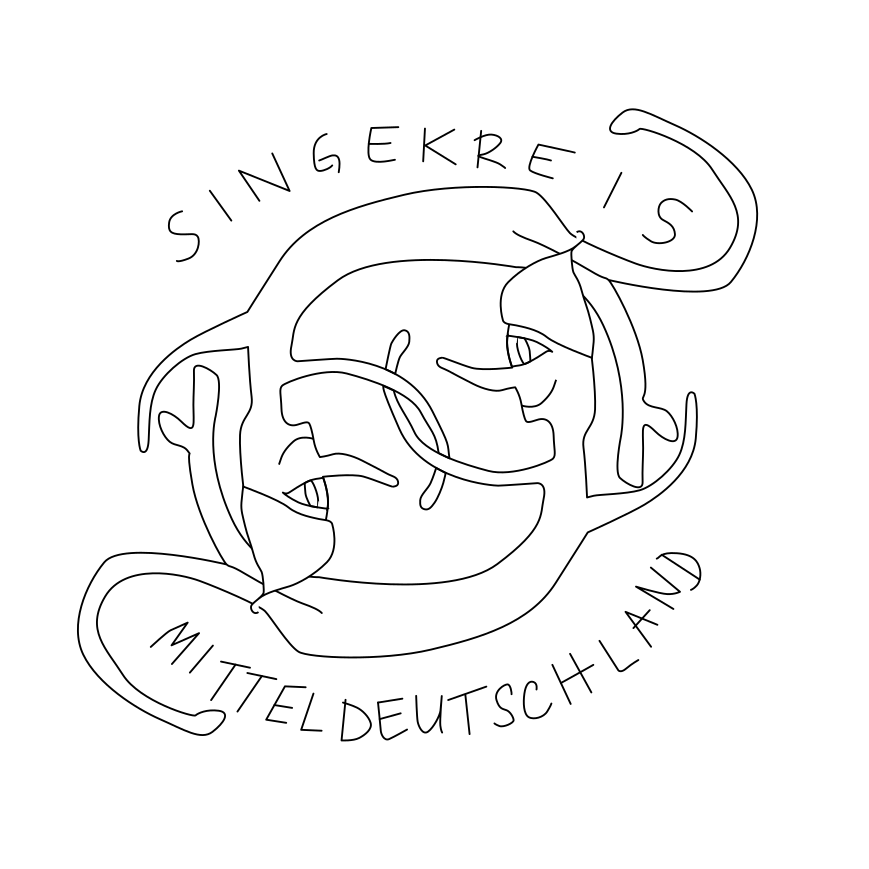
\includegraphics[width=.2\textwidth]{Rohdaten/Bilder/Singekreis.png}};
\end{tikzpicture} 
\ifthenelse{\equal{\Lizenz}{CC-BY-SA}}{
\begin{tikzpicture}[remember picture,overlay]
\node[anchor=south east,inner sep=5pt] at (current page.south east)
{
\includegraphics[width=.2\textwidth]{Rohdaten/Bilder/Lizenz.png}};
\end{tikzpicture} 
}{}

\begin{figure}[H]
\includepdf[trim=00mm 0mm 00mm 00mm ,pagecommand={},pages=1,width=1.3\textwidth]{Rohdaten/Noten/\Liedname _Noten.pdf}
\end{figure}
\vspace{\Abstand}

\begin{song} \noindent
%Hier kommen die Strophen rein. 
%für Akkorde: \chort{Akkord}{Wort über dem der Akkord stehen soll}
%Strophenzahl/Refrain: \textbf{Refrain:} 

%\textbf{2.}\chort{d}{Heißer} \chort{a}{Tee} und \chort{C}{Funken}\chort{F}{glut}



\end{song}


\end{document}
